\chapter{Approach}\label{ch:approach}
The PhD study adopts a socio-technical view towards the planning support systems in disaster response setting. Introducing a planning support to Disaster Response(DR) operations may create a socio-technical gap that need to be considered by system designers. We argue that the gap can be reduced by an appropriate interaction design supported by deep understanding socio-technical issues surrounding the planning support. In order to gain insight into the socio-technical issues, we adopted an ethnographic approach to explore and unpack interactions between human and planning support agent in disaster setting [missing?]. A serious mixed reality game (MRG) approach is adopted to create MRG AtomicOrchid(AO), which are used to simulate DR operations. Using the AO as a testbed, we outlined two potential interaction designs that are later deployed for field observations. In addition, efforts have been made to establish contact with professional response agency Rescue Global(RG), which leads two workshops entered on AO. Professional feedbacks on AO are collected from the workshops. \\

In this chapter, we will go through the Socio-technical Perspective of planning support system adopted by this PhD work (section ), followed by introduction serious mixed reality game (MRG) approach (section \ref{sec:SMRG}) and description of AtomicOrchid platform (section \ref{sec:AOdescription}). The section x will outline the two interaction designs that will be deployed to AO for field studies, and the section x gives an introduction of workshops with RG for professional feedbacks. \\


\section{Socio-technical Perspective of technology support for organizational work}\label{sec:sociotech}
This research is aimed to inform the design of planning support for organizational work conducted by responder teams. This PhD work adopts the a socio-technical view on the responder teams and their technological supporting systems. Integrating new technology support into a human organisation is a well-known challenge for socio-technical system design. In this PhD study, we anticipate the same challenge will be encountered for  introducing the planning support to disaster response operations.\\

The term socio-technical systems was originally coined by Emery and Trist (1960) to describe systems that involve a complex interaction between humans, machines and the environmental aspects of the work system. nowadays, this interaction is true of most enterprise systems. The corollary of this definition is that all of these factors  people, machines and context need to be considered when developing such systems. Within the context of CSCW the term stands for the recognition that aspects of both, technical as well as social subsystems, need to be considered when an organization introduces new technology and that there is a very complex relationship between the two. Social systems are characterized by phenomena such as communication and cooperation between human individuals, emergence of meaning systems, self-referential development of structures and In contrast, technical systems are characterized by artifacts, control, anticipation, state-transitions, pre- programmed adaptability, learning in respect to purposes which are determined from outside the system. Introducing a tech support system into an organization requires the technical system and a social system to be integrated, which causes lots of well-known problems in CSCW studies. \\

In the context of this study, the technology support is based on coalition formation algorithm, which requires a set of rigid inputs and produces task assignments. On the other hand, planning activities of responder teams are characterized by natural social processes such as communication, negotiation and cooperation. To support the responder teams with coalition formation technologies, the confrontation between social and technical is inevitable. \\

Some researchers have pointed out the existence of the inherent social technical gap, the great divide between what we know we must support socially and what we can support technically.  Some argued that human activity is highly flexible, nuanced, and contextualized and that computational entities such as information sharing, roles, and social norms need to be similarly flexible, nuanced, and contextualized. However, current technology support systems for organisations are often rigid and inflexible, failing to fully support the social world. Computer science is learning how to use techniques such as machine learning, user modelling to fill social-technical gap. It is hard to disprove that a technical solution is imminent. However, some argued that such a technical solution is unlikely, given that computer science, artificial intelligence (AI), information technology, and information science researchers have attempted to bridge the gap without success for at least 20 years. \\

We argue that the social aspect does not need to be fully supported through technological advance. A deep understanding of social issues and appropriate interaction design may lead to possible ``workaround'' of the socio-technical gap. Although technology support may be not fully integrated with the social aspects, We believe appropriate interaction design can reduce its negative impact on social process so that the benefits of technology can overweight its adverse social impact. \\

%The field of HCI achieved widespread recognition with its inherent focus on the importance of the interaction between people and technology at the fundamental level rather than just the design of the user interface. It explicitly recognised the importance of the roles of the social and technical aspects of work. HCI Literatures have identified a wide range of different methodologies that helps inform the development of socio-technical systems such as (1) Cognitive Work Analysis, (2) Ethnographic workplace analysis, (3) Human-centred design. Some of the recognised HCI methodologies underpin the serious game approach employed by this PhD work to understand socio-technical design space of agent-based planning support. [The switch to HCI is not smooth]\\

%[Field trials supported by interaction analysis  speech act]\\

%[Andy s literature review of 2004 supporting ethnographic study should be cited]\\


\section{Serious Mixed Reality Game as a testbed} \label{sec:SMRG}
One of our work`s main objectives is to study interaction and coordination situated in rich and `messy' real-world socio-technical settings. As it is difficult to deploy technological prototypes in real disasters, Serious game approach has been adopted by researchers to study technology interaction in disaster scenarios through game-like simulations, for example to prepare first responders for scenarios in which hazardous materials are involved (Losh, 2007). Abbasi et al. (2012) present a study in which locally distributed participants played the role of victims asking for help via social media in a simulated crisis, and participants that played the role of first responders used a coordination system to filter messages and mobilize the appropriate responder teams according to their assigned capabilities. (see section x).\\

The PhD work also adopts serious game approach to simulate a disaster response setting in which distributed responder teams are coordinated with a time and spatial constraints (see section x). More specifically, we create a Mixed Reality Game (MRG) as a testbed that enables studying team coordination, interaction and communication in a real-world disaster scenario whilst providing confidence in the efficacy of behavioural observations. The Mixed-reality games are recreational experiences that make use of pervasive technologies such as smart phones, wireless technologies and sensors with the aim of blending game events into a real world environment. The MRGs serve as a vehicle to study distributed interactions across multiple devices and ubiquitous computing environments `in the wild' (see section x).\\

The MRG testbed called AtomicOrchid (AO) simulates a radioactive incident. Participants of the game plays the role of responders `on the ground', coordinating with each other through GPS, map sharing and messaging, to achieve game objectives. The AO game system can be integrated with planning agents to support players on the ground, and the interaction layer between players and agents can be configured in different ways through modifications on the game interface. Through agent integration and interface modifications, we created three `probes' of agent planning support with different interaction designs. The three probes are then be used to conduct behavioural studies, which allows us to unpack human-agent interaction with different interaction designs.\\

\section{The AtomicOrchid Platform}\label{sec:AOdescription}
We designed and implemented the mixed reality game AtomicOrchid(AO) as a testbed for our field trials of different system interaction designs. The game involves field players on the ground (play as field responder) and online players in a control room (play as Headquarter).

\begin{figure}[h]
  \centering
  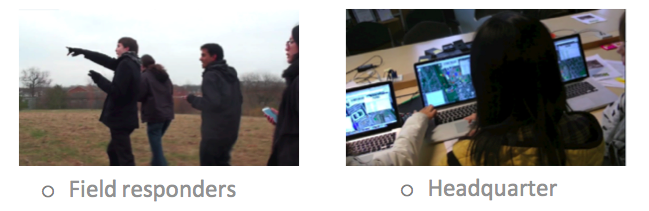
\includegraphics[width=1\textwidth]{img/approach/GameComponents}
  \caption{HQ and field players in AO}
  \label{fig:AOroles}
\end{figure}

In the following sections, we describe the game design including grounding of the design rationale,  iterative design process, and the system architecture.

\subsection{Game Design Rationale} \label{sec:gameRatinale}
The AtomicOrchid is based on the fictitious scenario of radioactive explosions creating expanding and moving radioactive clouds that pose a threat to responders on the ground (field responders), and the (virtual) targets to be rescued from around the game area. We chose a radiation scenario because other than disasters that cause physical devastation it poses an invisible threat, which creates the need to monitor the environment closely with sensing devices, and communicate frequently.\\

Field responders are supported by a centrally located headquarters (HQ) control room, staffed by coordinators who exchange messages with field players through an instant messaging style communication system. The messages are broadcasted, which means they are visible to all players. Whilst formal response teams tend to use radio to communicate (e.g., Toups et al., 2011) we chose text-based messages for its flexibility to support scenarios with many distributed (volunteer) field responders.\\

Core game mechanics are designed to allow us to explore specific aspects of team coordination. In particular, this is inspired by the real coordination challenge of resource and task allocation to coordinate spatially distributed resources and personnel\\

The game`s two-tiered organisational structure is derived from real world disaster response organisation and from NIMS (Homeland Security, 2008). The game`s HQ is loosely modelled on sector coordinators, whose role is to manage resources and communications between their assigned teams, and command and coordinate action within their sector (INSARAG, 2012). Field responders are modelled on team leaders and members. We ignore this distinction to simplify roles, assignments, and game mechanics.\\

\textbf{Responder roles and targets}. Each field responder is assigned one of four roles:\\

\begin{figure}[h]
  \centering
  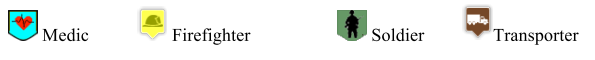
\includegraphics[width=1\textwidth]{img/approach/AOroles}
  \caption{The AO targets}
  \label{fig:AOroles}
\end{figure}

There are four types of (virtual) targets:\\

\begin{figure}[h]
  \centering
  
\includegraphics[width=1\textwidth]{img/approach/AOtargets}
  \caption{The AO targets}
  \label{fig:AOtargets}
\end{figure}

The objective of the field responders is to rescue as many targets as possible by `carrying' them to a drop off zone. To pick up and carry one of the target objects, two responders with particular appropriate roles are required in immediate proximity to the object. For example, a soldier and a transporter are required to pick up and carry fuel, and a medic and a soldier are required to pick up an animal (see figure \ref{fig:roleTargetMapping}).\\

\begin{figure}[h]
  \centering
  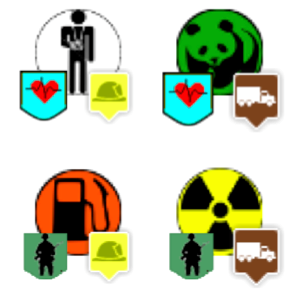
\includegraphics[width=0.3\textwidth]{img/approach/roleTargetMapping}
  \caption{Role target mapping}
  \label{fig:roleTargetMapping}
\end{figure}

The role-target mapping mechanic requires players to engage in resource coordination. Field responders have to engage in `agile teaming' forming, disbanding, relocating and re-forming in teams over the course of the game in order to complete the game objective. This is an example of what Toups et al call, information distribution (2011).\\

\textbf{The radioactive cloud}. The cloud is a danger zone that can incapacitate field responders. It imposes spatial and temporal constraints on task performance and well- being. The cloud is analogous to various spatial phenomena in disasters (e.g. spreading fires, diseases and floods). In require communication between HQ and field responders, the spatial position and movement of the cloud is only known to HQ. The cloud is shown in a heatmap style in the figure \ref{fig:cloud}. \\

\begin{figure}[h]
  \centering
  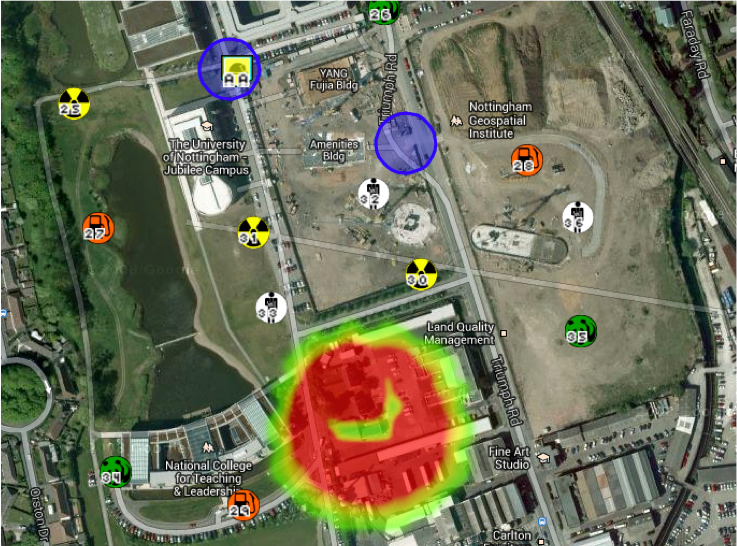
\includegraphics[width=0.8\textwidth]{img/approach/radioactiveCloud}
  \caption{The radioactive cloud}
  \label{fig:cloud}
\end{figure}

\textbf{Command-and-control structure}. The division of responsibility into HQ and field responders simulates a situation where volunteer responders are connected to a simple two level Command-and-control structure, similar to the real-time layer of the existing professional disaster response organizations (e.g., Chen et al., 2005).\\

\textbf{System interface}.System interface design is closely related to specific interaction designs, and it keeps evolving throughout three iterations of field trials. Therefore, the details of interface evolution is left to be introduced in the subsequent chapters (Chapter \ref{ch:studyone},\ref{ch:studytwo},\ref{ch:studythree}) of field trials. \\

\subsection{Iterative design and development}
Before the game is deployed for observational studies in this PhD work, the game went through a iterative design and development process to test, refine game concepts and system robustness. We briefly describe three cycles of iterative game design and evaluation before the system is ready for the first formal field study.\\

In the first iteration, we used a paper-based prototype to test and refine the core game mechanics. We recruited 12 participants, allocated one of four roles to them, and equipped them only with paper maps with locations of targets. They had to form different kinds of teams to retrieve the different kinds of boxes placed in the game area. The paper prototype demonstrated the demand for better support of situation awareness and communication to enable coordination.\\

The technology prototype was first tested with users in the second iteration. Users were equipped with the responder smartphone app to communicate, navi- gate, locate and pick up targets in teams formed according to role requirements. HQ was staffed by members of the research team. A pilot study was conducted with members of the public that visited an Open Day at a local university. A total of 20 members of the public tested the game in four ad-hoc game trials. The les- sons learned in the pilot study revealed problems with user interaction, network- ing, and game parameter tuning, which we subsequently addressed.\\

In the third iteration, we improved system stability and interface designs. We conducted a pilot study at the campus of another university, to test the system in place. The full-fledged study we report on here was conducted shortly thereafter.\\

\subsection{System Architecture}
The AtomicOrchid is based on the open-sourced geo-fencing game MapAttack that has been iteratively developed for a responsive, (relatively) scalable experience. Our mixed-reality game relies especially on real-time data streaming between client and server. The client-server architecture is depicted in figure \ref{fig:sysArchitecture}. Client-side requests for less dynamic content use HTTP. Frequent events, such as location updates and radiation exposure, are streamed to clients to avoid the overhead of HTTP. In this way, field responders are kept informed in near real-time.\\

\begin{figure}[h]
  \centering
  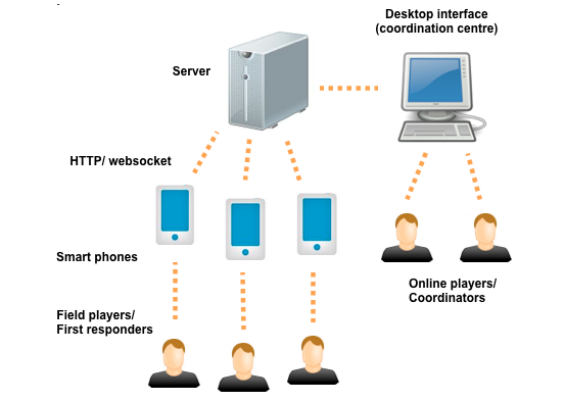
\includegraphics[width=1\textwidth]{img/approach/systemArchitecture}
  \caption{System Architecture}
  \label{fig:sysArchitecture}
\end{figure}

The platform is built using the Sinatra for Ruby, and state-of-the-art web technologies such as socket.io, node.js, redis and Synchrony for Sinatra, and the Google Maps API. Open source mobile client apps exist for iPhone and Android; we adapted an Android app to build the Mobile Responder App.\\


\subsection{The planning agent}
In study 2 and 3 (chapters \ref{ch:studytwo},\ref{ch:studythree}), planning agents are integrated into the AtomicOrchid to support player's planning activities. Two types of agent has be used in study 2 and 3 respectively. In what follows, we briefly describe technical details of the agent and system integration between AO and the agents.  \\

The coordination problem (described in section \ref{sec:gameRatinale}) is modelled using a Multi-Agent Markov Decision Process (MMDP) that captures the uncertainties of task execution, extending earlier work []. The modelling allows responder actions to be delayed or to fail during the rescue process. The MMDP modelling leads to a large search space, even with a small-sized problem. Hence, we devised an approximate solution to save computation time, which can be executed to support real time planning. The planning algorithm takes into account both time (cloud and human movement speed) and spatial (path planning for responders) constraints. The planning algorithm run by the planning agent produces high task allocations that minimise the travelling distance of first responders, and maximise the number of targets rescued. Before the agent was deployed to support human teams in the game setting, computational simulations were used to benchmark our MMDP algorithm against greedy and myopic methods (see figure \ref{fig:agentBenchmarking}). The results confirm that our algorithm produces efficient task allocations. It should the agents are developed by ORCHID Reseach partners from Southampton, more technical details of the planning agent is available in [JAMASS paper].\\

\begin{figure}[h]
  \centering
  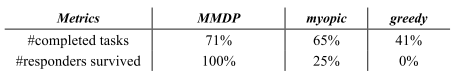
\includegraphics[width=1\textwidth]{img/approach/agentBenchmarking}
  \caption{Result for MMDP, Myopic and Greedy algorithms}
  \label{fig:agentBenchmarking}
\end{figure}

For integration, the agent is deployed on a separate server. It communicate with the AO game server through a pre-defined HTTP protocol (for details, see Appendix X). The agent takes game status from game server as input, which includes player's health, road connectivity, locations of players, targets and radioactive clouds. The output of the agent a set of task assignments likes `player A and player B, go to target C' (see figure \ref{fig:inputoutput}) . The task assignments are sent to the AO game server and present to game players. Detailed interaction design between human and the agents will be presented in Chapter \ref{ch:studytwo},\ref{ch:studythree}. In order to facilitate the different interaction designs, the input of the agents are slightly different between study 2 and study 3, which will be detailed in section \ref{sec:studyoneagent} , \ref{sec:studytwoagent}. \\

\begin{figure}[h]
  \centering
  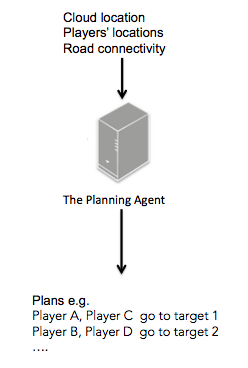
\includegraphics[width=0.5\textwidth]{img/approach/inputoutput}
  \caption{Input and output of the agents}
  \label{fig:inputoutput}
\end{figure}

\section{Three interaction designs}

[Working in progress ]
[Justify the relation between the three iterations]
- avoiding pitfalls that undermines observation of interaction arrangement
- HQ agent interaction can be parallel/ HQ FR interaction follows progressive design interaction
- The first iteraction: base case/ need to understand the organization before we do anything.

Based on serious game approach, three iterations of prototyping are planned to explore the interactional issues related to the socio-technical integration. The 3 different system prototypes are partially (loosely) inspired by the model of Level Of Automation (LOA) in the study of automation design. The LOA model has been developed to categorise systems into a linear spectrum according to degree of automation. There are several variations of the LOA models. One example is the two-dimensional LOA model proposed by Parasuraman (detailed in literature review section x). Several limitations of the LOA has been identified in chapter x. Most importantly, the LOA model has a focus on one-to-one operator-system interaction (e.g. autopilots, tele-oportation). It fails to capture complexity of the interactions in the context of technology support for organisational work. Therefore, it does not fit into the context of socio-technical system, which is the main focus of this research. \\

Despite the limitations, the terminologies that come with the model have been borrowed and adapted to inform the interaction design of three system prototypes in this research. \\

- Human Out of the Loop (HOuL)
HOuL represents the highest level of automation. HOuL system is supposed completely run independently. Human is replaced with machine, therefore no human system interaction is required. It is unlikely to be realized in a socio-technical system in which organisational work is mainly carried out by human and supported by technologies. \\

- Human In the Loop vs. Human On the Loop 
There is no precise definition for the term HuIL. Some automation researchers use the term to describe a system with high level of automation, which requires minimum level of human intervention. However, in this research, we use the term HuOL to describe this kind of system. Further, this research adapts definition of HuIL to represents medium level of automation. The HuIL system requires constant human interactions to achieve goal of socio-technical system.\\

Although the terms are originally used to describe degree of automation, this can also be used to inspire the interaction design of the system prototypes. new 

\section{Explore interaction designs with three AtomicOrchid studies}
- interaction designs 
- three game probes
- explore issues with 3 AtomicOrchid studies. 

\section{Collaboration with Professional Disaster Response Organisation}
In addition to the three observational studies of AtomicOrchid games, two workshops with a Rescue Global (a professional disaster response agency) was organised to get professional feedbacks about the AtomicOrhid system and planning support component. Because the contact with Rescue Global was established in very late stage of this PhD work, the feedbacks from Rescue Global (RG) workshop are not used to drive the development of AO simulation and interaction design, but to get an insight into similarity and difference between AO simulation and the real world disaster response(DR) operations, which help us understand limitations and strengths of our observational study.  The first RG workshop happened between study two and study three (section \ref{sec:RGworkshopone}). The In-the-loop AO probe was demonstrated to RG team and a discussion was organised to get feedbacks from RG. The second RG workshop happened after the study three (section x). It contains a hands-on session for RG to experience AO game, and the feedbacks are collected from discussions during and after the game session.\\

%\section{A framework of interactional issues}\label{sec:interactional}
%interaction techniques 
%[Which Interaction Technique Works When] refer to interaction techniques may refer to is a set of %interface widget design.

%We follows a process of interaction design documented in the [Designing interactions p 15], the process %is interactive, with a special focus on understanding issues and generating design implications . The %issues emerges in previous iterations will be feedback to next iterations. 

%interactional issues: 

%Interface aspects: tech dependent or not?
%interaction aspects: concerned with interaction patterns 
%Social aspects: Corncerned with what? 

%(Sedig, K.Parsons, P) pattern based approach.
%(Most interaction techniques literature reviewed so far is about study in visual representation. )
%(Interaction design, wiki)

\chapter{ Methodology To Investigating Human Agent Interaction}
This chapter takes an in-depth look at the methodology that underlies the empirical approach in the presented studies.This PhD study is aimed to conduct ethnographic-oriented field studies based on AO platform to generate descriptive results, which contains rich interactions among participants and system support. Ethnographic observations and interaction analysis are central to all three field studies, while group interviews are introduced as supplementing the in situ methods.\\

\section{Group interviews}
For all three field studies, group interviews were conducted with all participants after each game sessions. The interviews consists of open-ended questions with the aim to supplementing the field observation and interaction analysis with rich descriptions of participants' experiences of the game. Emergence of unanticipated issues and events was also fostered by asking open-ended questions, which in turn, are used to guide the interaction analysis of field observations.\\

\section{ Ethnomethodology perspective}
The method of observing participants in the field study is informed by Ethnomethodology (EM). Following the tradition of ethnography, EM seeks to explicate real-world organisation of works by adopting the naturalistic stance. The EM places methodological emphasis on rigorous description of the situated (i.e. local, observable) actions and practices (Suchman, 1987) in and through the contingent accomplishment of daily activities. The EM-informed ethnography arguably helps answering what might be regarded as an essential question in design: what to automate and (Crabtree et al. 3) what to leave to human skill, competence, judgement, experience and expertise. By producing description of the actions and practices in and through which the work `gets done' time and time by the members, The EM could inform the system design by uncovering what actions and activities we should therefore support.\\

For the the purpose of this thesis, the social situation the interaction with and around the planning support was argued to be a critical factor to understand how social organisation of work is achieved participants with the existence of a planning support system. Observation of the situated actions and practice employed by the participants was a key method in the field study. The use of the system was observed and filmed for later analysis. Video is widely recognised as an important resource for ethnographies around technology use (Crabtree et al., 2006). The next section will go through the method of video-based interaction analysis for unpacking the interactions observed in the field. \\

\section{Interaction Analysis}
Interaction analysis can be defined as an interdisciplinary method for empirical investigation of interaction of human beings with each other and with objects in their environments (Jordan and Henderson). In the context of HCI study, it is a method of analysing videorecordings of naturally occurring talk and activity, with the aim of uncovering, describing something of the order and organisation by which people interpret and interact with each other and with the things around them.\\

The Advantage of Interaction analysis lies in its ability to deal with actual details of technologically mediated interactions and allows technology developers to see exactly how technology fits (or doesn't fit) into current working practice. Other methods such as relies upon report from participants, rather than actual, reasoning and behaviour. The over-reliance on participants' report make those methods vulnerable to the problems of people producing post hoc rationalisations of actions, forgetting or incorrectly estimating aspects of behaviour, expressing ineffective attitudes, and generally lacking insight into the tacit procedures underlying much of their activity. Instead, interaction analysis can expose the practical reasoning activities of participant's themselves in a way which does not require them having to remember, justify or even know what they did. This effectively indicates how people think and make sense of technology they are using, in the performance of some task. However, interaction analysis is extremely time-consuming, which means it can only be carried out on small number of participants. The limitation makes it unsuitable for answering to very specific design questions and for examining the needs and behaviours of diverse groups of people. Furthermore, the generality of its findings may need to be established by other means.\\

For the purpose of this PhD work, interaction analysis is applied to the evaluation of game probes undergoing field trials in selected work settings of Disaster Response. In this case, the description generated by interaction analysis could expose information on the sequential organisation of technologically and socially mediated activities, which in turn, reveals how the activities can be supported.\\
